%\subsection{Фундаментальные принципы черенковских детекторов}
%
%% Источник - http://nuclphys.sinp.msu.ru/enc/e186.htm
%
%\begin{minipage}[t]{0.495\textwidth}
%В основе черенковских детекторов лежит эффект Вавилова--Черенкова, который заключается в том, что заряженная частица испускает свет при движении в прозрачной среде со скоростью $\vartheta$ большей скорости света в этой среде, равной $c/n$, где $c$~---~скорость света в вакууме, а $n$~---~показатель преломления среды. Порог свечения: \\
%\begin{spacing}{1.5}
%{\centering
%$\beta = \frac{\vartheta}{c} \geq \frac{1}{n}$ \\}
%\end{spacing}
%Волновой фронт этого излучения представляет собой поверхность конуса, вершиной которого является частица, а осью --- её траектория. Угол раствора конуса $\theta$ фиксирован и определяется скоростью частицы $\vartheta$ и свойствами среды исходя из следующих соотношений: \\
%\begin{spacing}{1.5}
%{\centering
%$AC = \vartheta t = \frac{\vartheta c t}{c} = \beta c t$ \\
%$AB = \frac{c}{n} t$ \\
%$cos\theta = \frac{AB}{AC} = \frac{ct/n}{\beta c t} = \frac{1}{\beta n}$ \\}
%\end{spacing}
%\end{minipage}
%\begin{minipage}[t]{0.495\textwidth}
%\begin{figure}[H]
%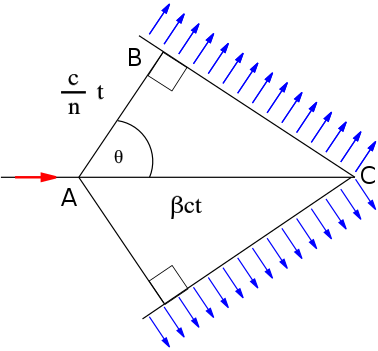
\includegraphics[width=0.9\textwidth]{pictures/Cherenkov.png}
%\caption{Геометрия черенковского излучения.}
%\label{fig:CherenkovGeo}
%\end{figure}
%\end{minipage}
%
%Черенковское излучение находится в области видимого света и ближнего ультрафиолета, что даёт возможность регистрировать его различными фотодетекторами.
%
%\subsubsection{-----------------------}
%
%За счёт того, что наличие свечения определяется скоростью, а не импульсом или энергией, связанными со скоростью через массу, предоставляется возможность идентификации частиц. При той же энергии более лёгкая частица будет иметь больше скорость, а более тяжёлая --- меньше скорость, причём возможно, что ниже порога свечения.
%Правильным подбором материала радиатора \todo ... выбирается диапазон энергий
%
%\subsection{Черенковские детекторы}
%
%% Источник - http://nuclphys.sinp.msu.ru/experiment/detectors/cherenk.htm
%
%Эффект Вавилова--Черенкова применяется в физике частиц для построения трёх типов детекторов: пороговых черенковских счётчиков, дифференциальных черенковских счётчиков \todo,\todo и черенковских детекторов кольцевого изображения (RICH-детекторов). 
%
%Пороговый черенковский счётчик служит для регистрации частицы, имеющей скорость выше порога свечения. Т.к. порог определяется материалом радиатора, существует возможность простейшей идентификации частиц путём установки двух или более различных радиаторов на пути пучка. Если, например, имеется два подобранных радиатора, то частицы одного типа будут светиться только в обоих, частицы другого типа --- только в одном, а третьи --- ни в одном.
%
%\begin{minipage}[t]{0.495\textwidth}
%\begin{figure}[H]
%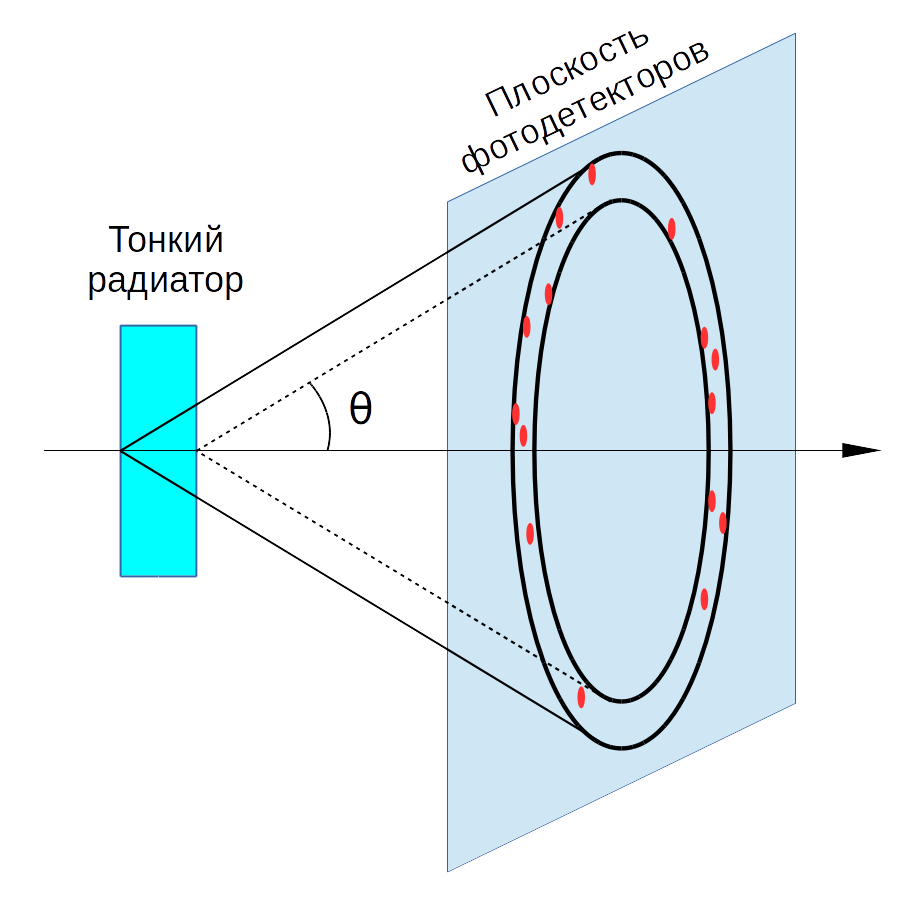
\includegraphics[width=0.9\textwidth]{pictures/RICH_scheme.png}
%\caption{Схема RICH-детектора \\с квазифокусировкой.}
%\label{fig:RICHbasic}
%\end{figure}
%\end{minipage}
%\begin{minipage}[t]{0.495\textwidth}
%\begin{figure}[H]
%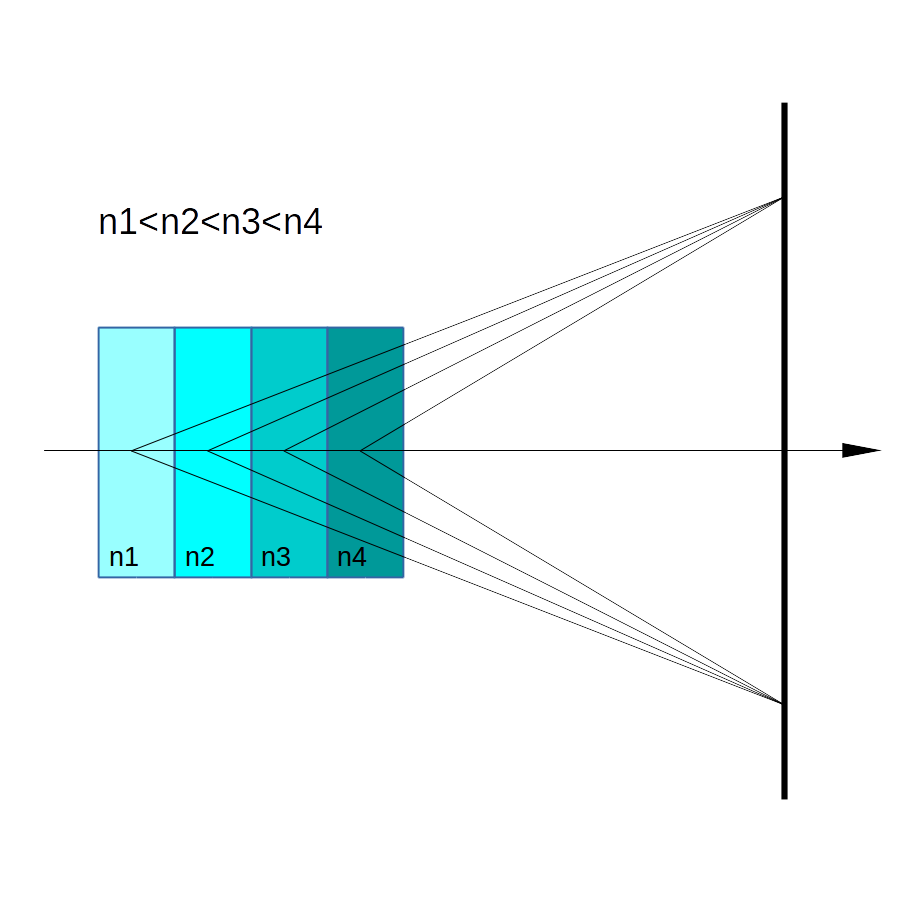
\includegraphics[width=0.9\textwidth]{pictures/RICH_layered.png}
%\caption{Схема RICH-детектора \\с многослойным радиатором.}
%\label{fig:RICHlayered}
%\end{figure}
%\end{minipage}
%
%Дифференциальные черенковские счетчики регистрируют частицы в определенном интервале скоростей. Т.к. черенковский угол пропорционален скорости, присутствует возможность построения оптической системы, разделяющей частицы, летящие под разными углами, то есть с разными скоростями. В зависимости от того, какая группа фоточувствительных элементов зарегистрировала свет, делается вывод о скорости пролетевшей частицы.
%
%RICH-детекторы используют тот факт, что черенковский свет излучается под постоянным углом $\theta$ к траектории частицы. Отсюда следует, что черенковский свет, возможно после оптической фокусировки, формирует изображение кольца в некоторой плоскости. RICH-детекторы можно классифицировать по нескольким признакам. По способу фокусировки RICH-детекторы можно разделить на три типа: с прямой фокусировкой, со сферическим или параболическим зеркалом и DIRC-детекторы.
%
%\textbf{Перетасовать!}
%(По радиатору:) В качестве радиатора может использоваться газ (самые распространённые --- $CO_{2}$, $CF_{4}$, $C_{4}F_{10}$), жидкий или твёрдый материал, как частный случай --- аэрогель.
%(По фотодетектору:) Микроканальные пластины, ФЭУ, фотодиоды, ...
%\textbf{Перетасовать!}
%
%Если поставить на пути черенковского света плоскость фотодетекторов, то, с учётом того, что радиатор имеет конечную длину, на ней образуется изображение кольца. На~\figref{fig:RICHbasic} показана схема RICH-детектора с квазифокусировкой (прямой фокусировкой), в которой радиатор обычно выбирается тонким и с большим показателем преломления. Это позволяет регистрировать кольцевое изображение напрямую, без какой-либо дополнительной оптической подсистемы. Для того чтобы преодолеть проблему малого выхода фотонов в небольшом объёме радиатора применяют слоистые радиаторы (см.~\figref{fig:RICHlayered}), в которых каждый следующий слой имеет больший показатель преломления, и следовательно, больший угол черенковского света.
%
%Во втором варианте RICH-детекторов оптический материал радиатора одновременно используется и как черенковский радиатор, и как светопровод (см.~\figref{fig:DIRC}). Радиатор (например кварц) имеет прямоугольную форму. За счет этого, фотоны черенковского излучения, испущенные под углом $\theta$, распространяются вдоль пластины за счет полного внутреннего отражения с сохранением этого угла до самого торца пластины, где расположен позиционно-чувствительный фотоприёмник. Такой тип детекторов называют DIRC-детекторами (Detection of Internally Reflected Cherenkov light).
%
%\begin{figure}[H]
%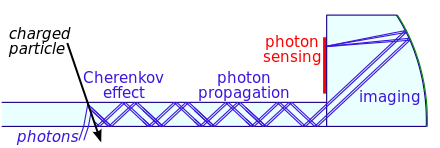
\includegraphics[width=0.7\textwidth]{pictures/DIRC.png}
%\caption{Принцип DIRC-детекторов.}
%\label{fig:DIRC}
%\end{figure}
%
%\begin{minipage}[t]{0.495\textwidth}
%\begin{figure}[H]
%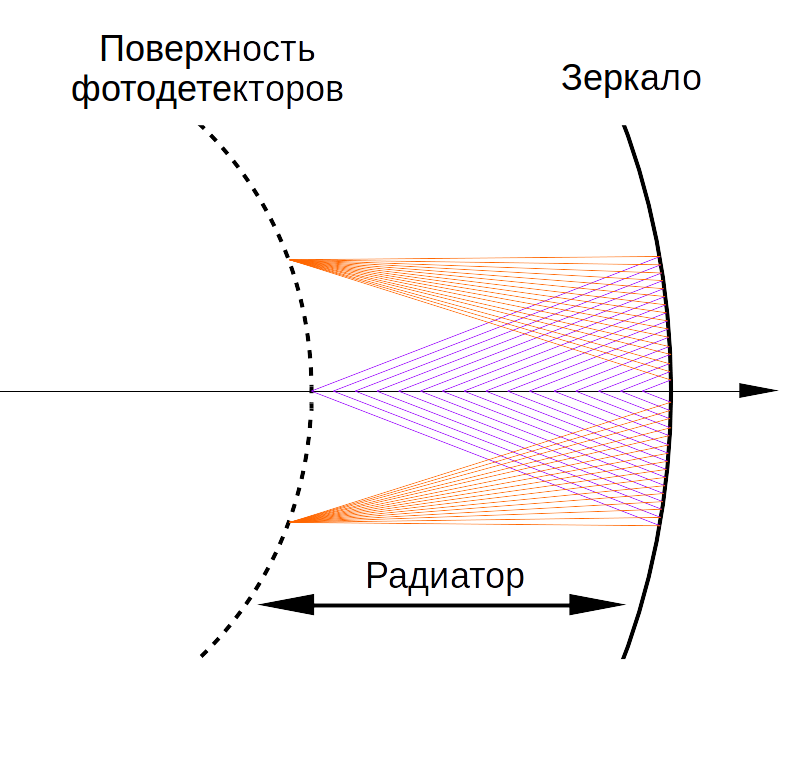
\includegraphics[width=0.9\textwidth]{pictures/RICH_spherical.png}
%\caption{Схема RICH-детектора \\со сферическим зеркалом.}
%\label{fig:RICHspherical}
%\end{figure}
%\end{minipage}
%\begin{minipage}[t]{0.495\textwidth}
%Если в качестве радиатора используется газ, для того чтобы излучалось достаточное количество фотонов, толщина радиатора должна быть довольно большой. В этом случае для фокусировки используются сферические или параболические зеркала. В таком детекторе радиатор находится между двумя сферическими поверхностями (см.~\figref{fig:RICHspherical}). Наружная --- сферическое зеркало радиуса $R$. Источник частиц находится в центре сферы. На внутренней сфере радиуса $R/2$ устанавливаются фотодетекторы. Отраженное от зеркала черенковское излучение фокусируется на внутреннюю сферу, образуя кольцо радиусом $r = R/2 \times tg(\theta)$. Для того чтобы вывести фотодетекторы из аксептанса детектора зеркало может быть повёрнуто, а иногда применяют и дополнительные плоские зеркала (см. \todo). Из конструктивных соображений поверхность фотодетекторов нередко выполняют плоской или собирают из нескольких плоских модулей.
%Так, например, в CBM RICH используются оба упомянутых приёма --- фокусная цилиндрическая поверхность аппроксимируется набором плоских модулей МА~ФЭУ, расположенных за пределом аксептанса детектора, а фокусировка выполняется одним отражением от сферических зеркал, размещённых в стороне от пучка и повёрнутых на некоторый угол.
%\end{minipage}